%ब

\section{Solution 2:  Metadata as a Top Row} \label{s:design-sol2}


In Solution~2,   metadata is embedded with the actual data and exists in the
same column family as the actual data which is similar to Solution~1. 
% where metadata is stored within the same column family. 
However,  in this solution   metadata is saved only once in the column family as
a top row (i.e. the first super column in a column family) with the unique
\texttt{RowId} '\texttt{-1}'.  This top row has only the \texttt{Metadata} 
column containing the metadata information as its value while the rest of the
super columns in the same column family have different columns containing the
actual data.  This design is possible since Cassandra allows rows to have
different number of columns within a column family.  The \texttt{Metadata}
column is similar to the Solution~1 as shown in Figure~\ref{fd:Metadata-Column}.  Thus,  for
each column family,  its metadata exists only once as a single row and is common
for all its super columns.  In the University example, the  \texttt{Student}
column family has the metadata  stored as a top row as  shown in
Figure~\ref{fd:Metadata-Solution2}.  
% This approach helps preserve the dependency
% information while also making it easily accessible for the referential integrity 
% validations. 
		 
	\begin{figure}[h]  
		\centering 
		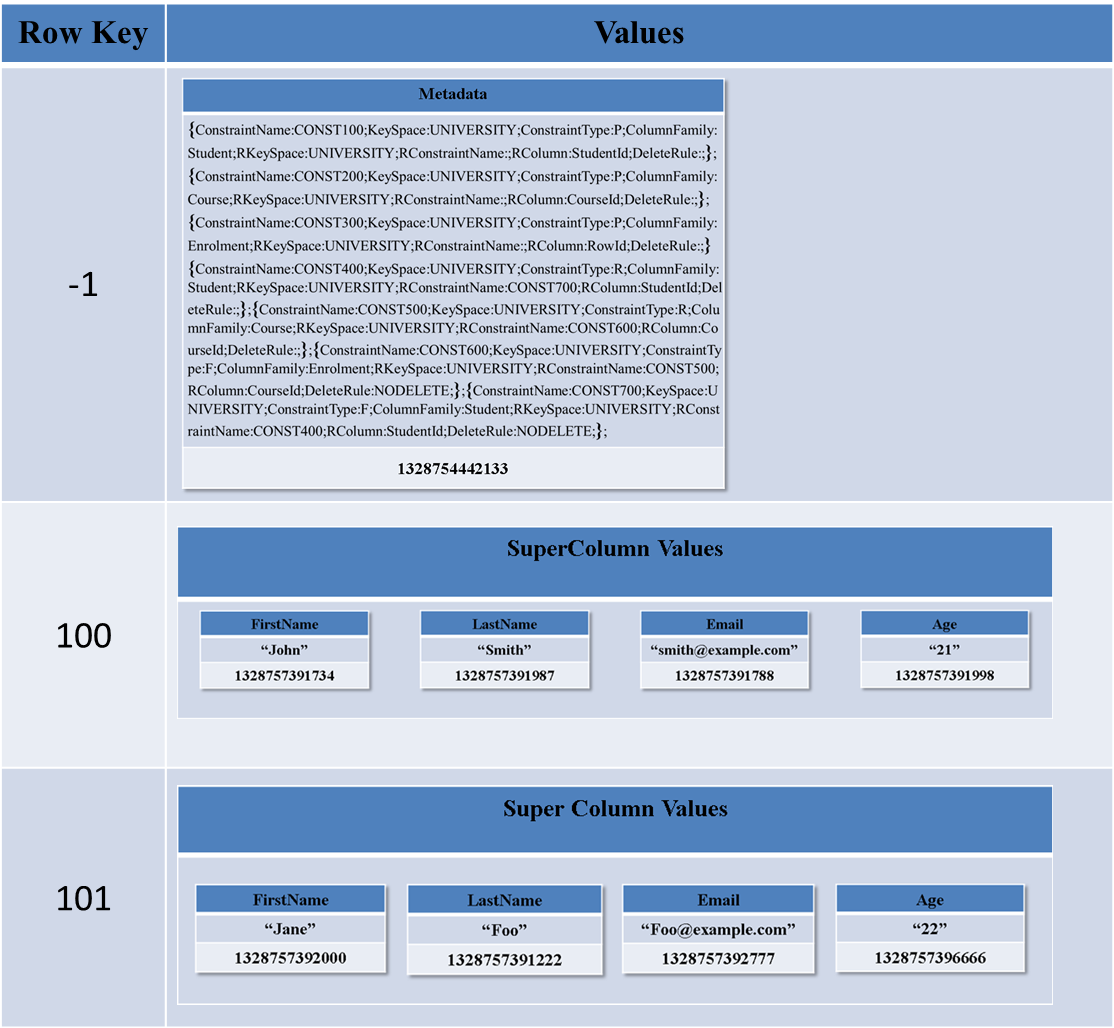
\includegraphics[width=.8\textwidth]{./figure/Solutions/Sol2-MD-ColumnFamily.png}
		\caption{Metadata storage in Solution 2}\label{fd:Metadata-Solution2}
	\end{figure}
		

In this solution, metadata  for each column family contains all the constraints
belonging to the keyspace. The metadata contains special characters
'\texttt{\{}',  '\texttt{\}}', '\texttt{;}' and '\texttt{:}' to distinguish all
the constraints and its different parts and values, which is similar to
Solution~1. Thus, in this Solution, the metadata for \texttt{Student}  contains
all the constraints (as listed in Figure~\ref{fd:Metadata-Constraints}) as its
metadata in the top row as shown in Figure~\ref{fd:Metadata-Solution2}.


% Consider \texttt{Enrolment}  which is a child entity with parent entities
% \texttt{Student} and \texttt{Course} (Figure~\ref{}).  Its metadata thus contains
% its \ac{PK} constraint \texttt{CONST300} and the \ac{FK} constraints
% \texttt{CONST400} and \texttt{CONST500}.  Since \texttt{Student} is a child
% entity it  stores its \ac{PK} constraint \texttt{CONST100} and its \ac{FK}
% constraint \texttt{CONST700}.  Similarly,  \texttt{Course} stores its \ac{PK} and
% respective \ac{FK} constraints. 
% 
% 	\begin{figure}
% 	\todo{ Insert metadata top row figure for Enrolment}
% 	\end{figure}
% 	Thus,  the metadats describes which is the
% 	primary key for the entity and the \ac{FK} constraints show which child entities dependent on the
% 	entity.  The \ac{FK} constraints are particularly useful to . 
	
The motivation behind this solution is to overcome the redundancy of metadata
storage in Solution~1.  In Solution~1,  metadata is stored in every super column
of a column family and replicated across the cluster along with the column
family.  Solution~2 reduces this redundancy and centralises the metadata as a top
row within the column family.  Thus,  when metadata is large, lesser space is
consumed since it is not replicated as widely as in Solution~1. 
% In other words, the aim of this design was to reduce the redundancy of metadata in the column
% family whilst having metadata accessible to all the nodes by having it embedded
% with the actual data. 
Furthermore,  this solution  ensures that, when changes are made to the
metadata, the actual data is not accessed and only the
column family  is accessed to fetch the top row containing the metadata. 










